

\tikzset{every picture/.style={line width=0.75pt}} %set default line width to 0.75pt        

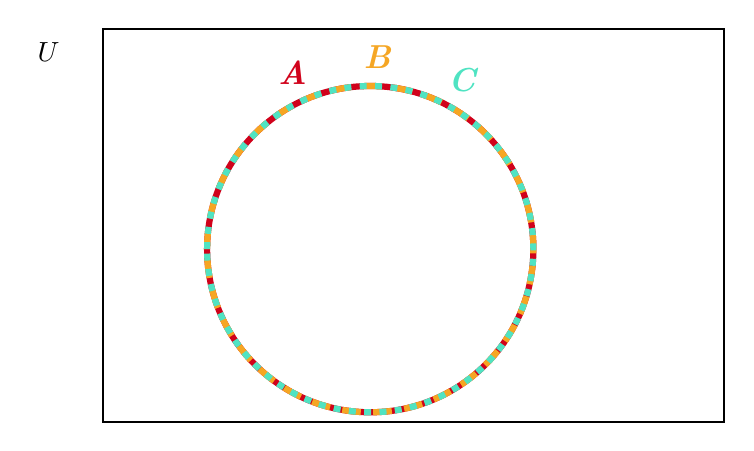
\begin{tikzpicture}[x=0.75pt,y=0.75pt,yscale=-1,xscale=1,scale= 0.8]
%uncomment if require: \path (0,256); %set diagram left start at 0, and has height of 256

%Shape: Rectangle [id:dp03257259596647377] 
\draw  [color={rgb, 255:red, 0; green, 0; blue, 0 }  ,draw opacity=1 ] (147,6) -- (521,6) -- (521,243) -- (147,243) -- cycle ;
%Shape: Circle [id:dp3347773199535533] 
\draw  [color={rgb, 255:red, 208; green, 2; blue, 27 }  ,draw opacity=1 ][line width=2.25]  (209.5,138.75) .. controls (209.5,84.49) and (253.49,40.5) .. (307.75,40.5) .. controls (362.01,40.5) and (406,84.49) .. (406,138.75) .. controls (406,193.01) and (362.01,237) .. (307.75,237) .. controls (253.49,237) and (209.5,193.01) .. (209.5,138.75) -- cycle ;
%Shape: Circle [id:dp7644399651294971] 
\draw  [color={rgb, 255:red, 245; green, 166; blue, 35 }  ,draw opacity=1 ][dash pattern={on 6.75pt off 4.5pt}][line width=2.25]  (209.5,138.75) .. controls (209.5,84.49) and (253.49,40.5) .. (307.75,40.5) .. controls (362.01,40.5) and (406,84.49) .. (406,138.75) .. controls (406,193.01) and (362.01,237) .. (307.75,237) .. controls (253.49,237) and (209.5,193.01) .. (209.5,138.75) -- cycle ;
%Shape: Circle [id:dp3198096122185099] 
\draw  [color={rgb, 255:red, 80; green, 227; blue, 194 }  ,draw opacity=1 ][dash pattern={on 2.53pt off 3.02pt}][line width=2.25]  (209.5,138.75) .. controls (209.5,84.49) and (253.49,40.5) .. (307.75,40.5) .. controls (362.01,40.5) and (406,84.49) .. (406,138.75) .. controls (406,193.01) and (362.01,237) .. (307.75,237) .. controls (253.49,237) and (209.5,193.01) .. (209.5,138.75) -- cycle ;

% Text Node
\draw (261,33) node [scale=1,color={rgb, 255:red, 245; green, 166; blue, 35 }  ,opacity=1 ] [align=left] {\textit{\textcolor[rgb]{0.82,0.01,0.11}{{\large \textbf{A}}}}};
% Text Node
\draw (107,16) node  [align=left] {$ $};
% Text Node
\draw (114,20) node   {$U$};
% Text Node
\draw (312,23) node [scale=1,color={rgb, 255:red, 245; green, 166; blue, 35 }  ,opacity=1 ] [align=left] {\textit{\textbf{{\large \textcolor[rgb]{0.96,0.65,0.14}{B}}}}};
% Text Node
\draw (363,37) node [scale=1,color={rgb, 255:red, 80; green, 227; blue, 194 }  ,opacity=1 ] [align=left] {{\large \textbf{\textit{\textcolor[rgb]{0.31,0.89,0.76}{C}}}}};


\end{tikzpicture}